
%% 
%% Copyright 2007, 2008, 2009 Elsevier Ltd
%% 
%% This file is part of the 'Elsarticle Bundle'.
%% ---------------------------------------------
%% 
%% It may be distributed under the conditions of the LaTeX Project Public
%% License, either version 1.2 of this license or (at your option) any
%% later version.  The latest version of this license is in
%%    http://www.latex-project.org/lppl.txt
%% and version 1.2 or later is part of all distributions of LaTeX
%% version 1999/12/01 or later.
%% 
%% The list of all files belonging to the 'Elsarticle Bundle' is
%% given in the file `manifest.txt'.
%% 
%% Template article for Elsevier's document class `elsarticle'
%% with harvard style bibliographic references
%% SP 2008/03/01

\documentclass[preprint,9pt]{elsarticle}

%% Use the option review to obtain double line spacing
%documentclass[authoryear,preprint,review,12pt]{elsarticle}

%% Use the options 1p,twocolumn; 3p; 3p,twocolumn; 5p; or 5p,twocolumn
%% for a journal layout:
%% \documentclass[final,1p,times,authoryear]{elsarticle}
%% \documentclass[final,1p,times,twocolumn,authoryear]{elsarticle}
%% \documentclass[final,3p,times,authoryear]{elsarticle}
%%\documentclass[final,3p,times,twocolumn,authoryear]{elsarticle}
%% \documentclass[final,5p,times,authoryear]{elsarticle}
%% \documentclass[final,5p,times,twocolumn,authoryear]{elsarticle}

%% For including figures, graphicx.sty has been loaded in
%% elsarticle.cls. If you prefer to use the old commands
%% please give \usepackage{epsfig}

%% The amssymb package provides various useful mathematical symbols
\usepackage{amsmath,amssymb,bm}
%\usepackage[dvips,colorlinks=true,citecolor=green]{hyperref}
\usepackage[colorlinks=true,citecolor=green]{hyperref}
%% my added packages
\usepackage{float}
\usepackage{csquotes}
\usepackage{verbatim}
\usepackage{caption}
\usepackage{subcaption}
\usepackage{booktabs} % for nice tables
\usepackage{csvsimple} % for csv read
\usepackage{graphicx}
\usepackage{url}
%\usepackage[outdir=//odroid-sensors/sensors/aidd/reports/journal_papers/MSSP_Paper/Figures/]{epstopdf}
%\usepackage{breqn}
\usepackage{multirow}
% matrix command 
\newcommand{\matr}[1]{\mathbf{#1}} % bold upright (Elsevier, Springer)
% vector command 
\newcommand{\vect}[1]{\mathbf{#1}} % bold upright (Elsevier, Springer)
\newcommand{\ud}{\mathrm{d}}
\renewcommand{\vec}[1]{\mathbf{#1}}
\newcommand{\veca}[2]{\mathbf{#1}{#2}}
\renewcommand{\bm}[1]{\mathbf{#1}}
\newcommand{\bs}[1]{\boldsymbol{#1}}
% limits underneath
\DeclareMathOperator*{\argmin}{arg\,min}
\DeclareMathOperator*{\argmax}{arg\,max}

\graphicspath{{Figures/}}

%% The amsthm package provides extended theorem environments
%% \usepackage{amsthm}
%% The lineno packages adds line numbers. Start line numbering with
%% \begin{linenumbers}, end it with \end{linenumbers}. Or switch it on
%% for the whole article with \linenumbers.
%% \usepackage{lineno}
\journal{Mechanical Systems and Signal Processing}

\begin{document}
	\begin{frontmatter}
		\addcontentsline{toc}{section}{References}
		%% Title, authors and addresses
		%% use the tnoteref command within \title for footnotes;
		%% use the tnotetext command for theassociated footnote;
		%% use the fnref command within \author or \address for footnotes;
		%% use the fntext command for theassociated footnote;
		%% use the corref command within \author for corresponding author footnotes;
		%% use the cortext command for theassociated footnote;
		%% use the ead command for the email address,
		%% and the form \ead[url] for the home page:
		%% \title{Title\tnoteref{label1}}
		%% \tnotetext[label1]{}
		%% \author{Name\corref{cor1}\fnref{label2}}
		%% \ead{email address}
		%% \ead[url]{home page}
		%% \fntext[label2]{}
		%% \cortext[cor1]{}
		%% \address{Address\fnref{label3}}
		%% \fntext[label3]{}
		
		\title{Full Wavefield Processing by Using FCN for Delamination Detection}
		
		%% use optional labels to link authors explicitly to addresses:
		%% \author[label1,label2]{}
		\address[IFFM]{Institute of Fluid Flow Machinery, Polish Academy of Sciences, Poland}
		
		\author{Abdalraheem A. Ijjeh\fnref{IFFM}}
		\author{Saeed Ullah \fnref{IFFM}}
		\author{Pawel Kudela\corref{cor1}\fnref{IFFM}}
		\ead{pk@imp.gda.pl}
		%\ead{pfiborek@imp.gda.pl}
		%\author{Tomasz Wandowski \fnref{IFFM}}	
		
		\cortext[cor1]{Corresponding author}
		
		\begin{abstract}
		A novel full wavefield processing method by using fully convolutional neural networks is presented.
The full wavefield of propagating Lamb waves in the fibre-reinforced composite plate was simulated by the parallel spectral element method.
It resembles a full wavefield measurements acquired on a surface of the plate by the scanning laser Doppler vibrometer.
The aim of the proposed technique is an identification of delamination location, size and shape.
It is achieved by pixel-wise image segmentation by using the end-to-end approach.
It is possible because of the large dataset of Lamb wave propagation patterns resulting from interaction with delaminations of random location, size and shape.
It is demonstrated that the proposed method, tested on numerical data, is performing better than conventional adaptive wavenumber filtering method which was developed in previous work.
Moreover, it enables better automation of delamination identification so that the damage map can be created without user intervention.
The method was also tested on experimental data acquired on the surface of the specimen in which delamination was artificially created by a Teflon insert.
The obtained results with the deep learning approach show its capability to predict the delamination in the numerically generated dataset with high accuracy compared to the conventional damage detection approach. Furthermore, the deep learning model shows the ability to generalize to a further experiential set.
		\end{abstract}
		
		\begin{keyword}
			%% keywords here, in the form: keyword \sep keyword
			Lamb waves \sep structural health monitoring \sep non-destructive testing \sep delamination identification \sep deep learning \sep  fully convolutional neural networks 
			%% PACS codes here, in the form: \PACS code \sep code
			
			%% MSC codes here, in the form: \MSC code \sep code
			%% or \MSC[2008] code \sep code (2000 is the default)
			
		\end{keyword}
		
	\end{frontmatter}
	%% main text

%%%%%%%%%%%%%%%%%%%%%%%%%%%%%%%%%%%%%%%%%%%%%%%%%%%%%
\section{Introduction}
%%%%%%%%%%%%%%%%%%%%%%%%%%%%%%%%%%%%%%%%%%%%%%%%%%
Composite materials have a wide range of applications in various industries, due to their characteristics such as high strength, low density, resistance to fatigue and corrosion.  
However, damage can occur in composite materials due to impacts resulting from the lack of reinforcement in the out-of-plane direction~\cite{Francesconi2019}.
In particular, laminated composite materials are more sensitive to damage in the form of delamination due to weak transverse tensile and interlaminar shear strengths.
Delamination can alter the compression strength of composite laminate, and gradually affect the composite to encounter failure by buckling. 
Delaminations can seriously decrease the performance of composite structures, accordingly, delamination detection in its early stages can significantly help to avoid catastrophic structural collapses.

One of the conventional techniques for damage identification for non-destru\-ctive testing (NDT) involves arrays of transducers that can be mounted or embedded in the structures for registering the response of the guided wave propagation.
%However, damage identification regarding structures with curved and deformable geometry can be inaccurate when using an array of transducers.
However, damage influence maps resulted from processing of signals registered by the array of transducers have low resolution, due to the small number of sensing points. 
Accordingly, this issue of low-resolution damage influence map can be solved by utilising a Scanning Laser Doppler Vibrometry (SLDV), which is a non-contact technique dedicated to full wavefield measurements of vibration and guided wave propagation.
%Moreover, the delamination location plays a key role in its identification i.e. delamination located at the edges or the corners of a structure are considered difficult scenarios due to a reflected signals from these locations have similar characteristics of those reflected from damage.
%Therefore, utilising SLDV for acquiring signals to produce a higher resolution influence map will be more beneficial than only using a transducers array. 
The measurements are conducted on a dense mesh of measurement points spanned over the area of the investigated structure.
Consequently, SLDV produces a full wavefield of measurements with high resolution of damage influence maps which can significantly improve the process of damage detection and localisation~\cite{Michaels2007,Park2014,Tian2015a,Kudela2015}.
Full wavefield processing techniques even allow for damage size estimation~\cite{Girolamo2018a,Kudela2018} which is difficult to perform in case of transducer arrays, especially for composite structures.
Therefore, the latter methods are evaluated mostly for damage detection and localisation in metallic structures~\cite{Michaels2008a,Huang2018a,Wang2020}.

Certain algorithms such as the time reversal algorithm can benefit from combining piezoceramic transducers (as actuators) with SLDV for sensing~\cite{Girolamo2018a, Miniaci2019}.
    
Conventional damage detection and localisation methods focus on patterns extraction from registered measurements and accordingly make decisions based on these patterns~\cite{Gul2009}. 
Moreover, conventional methods for pattern recognition require feature selection and classification (handcrafted features). 
These conventional methods can perform efficient damage detection, however, these methods depend on selected features from their scope of measurement.
Accordingly, introducing new patterns will cause them to fail in detecting the damage.
Furthermore, these methods could fail in detecting damage when dealing with big data requiring a complex computation of damage features~\cite{Gulgec2019}.
Perhaps the most challenging part for damage detection is determining the unknown relationship between registered measurements and damage patterns~\cite{Gulgec2019}. 
    
The accelerated progress in the field of artificial intelligence (AI) technologies in recent years, and mainly in deep learning, revealed new dimensions for solving problems and offered the opportunity for being implemented and integrated with the NDT and further with structural health monitoring (SHM) approaches.
Therefore, issues regarding data preprocessing and feature extraction can be handled when applying deep learning techniques. 
Nowadays, end-to-end approaches are developed, in which the whole unprocessed data are fed into the model, hence, it will learn by itself to recognise the patterns and detect the damage.
    
%%%%%%%%%%%%%%%%%%%%%%%%%%%%%%%%%%%%%%%%%%%%%%%%%%%%%
Deep learning techniques have widely been utilised for the inspection and maintenance of civil infrastructure and have shown very promising results~\cite{cha2017b, Lin2017a, liu2019computer, beckman2019deep, choi2019sddnet}. 
It has also been successfully applied for various fault diagnosis based tasks in rotating machinery~\cite{janssens2016convolutional}. 
For instance, Cha et al.~\cite{cha2017b} proposed a computer vision-based method using deep Convolutional Neural Network (DCNN) for the detection of concrete cracks. 
They compared their Convolutional Neural Network (CNN) based approach with traditional edge detection techniques such as Sobel and Canny methods and showed that their proposed model achieved quite better results and is very suitable for finding concrete cracks in realistic situations. 
Lin et al.~\cite{Lin2017a} developed an automatic damage feature extraction DCNN model and their results showed that DCNN outperformed conventional methods in realistic situations. 
Choi and Cha~\cite{choi2019sddnet} developed an encoder-decoder based semantic segmentation damage detection network (SDDNet), a real-time segmentation method based on CNN. 
SDDNet was inspired by a DenseNet and DeepLabV3+~\cite{chen2018encoder}. 
Liu et al.~\cite{liu2019computer} applied the U-Net network structure based on fully convolutional networks (FCN) for the purpose of identifying the locations of cracks in the raw input images of civil infrastructure under different conditions such as messy background, illumination, width of the cracks, etc. 
They compared their trained U-Net model with DCNN based method and found that the U-Net based model shown better performance as compared to DCNN in various circumstances.  
Beckman et al.~\cite{beckman2019deep} proposed a faster region-based CNN (Faster R-CNN)-based concrete spalling damage detection approach with the use of an inexpensive depth sensor for quantifying multiple instances of spalling. The Faster R-CNN enables the detection, localisation, and quantification of the amount of concrete spalled from a concrete element automatically. 
The Faster R-CNN provides a bounding box for the detection and localisation of defects. 
Janssens et al. ~\cite{janssens2016convolutional} developed a CNN based feature learning method for autonomously detecting different faults in rotating machinery with the use of vibration data. 
The input to the CNN modal was a discrete Fourier Transform of the two accelerometers. 
They compared their CNN based model with the classical feature-engineering based method which employs manually engineered features and a random forest classifier. 
They showed that their CNN based model outperformed the classical feature-engineering based approach. 

%%%%%%%%%%%%%%%%%%%%%%%%%%%%%%%%%%%%%%%%%%%%%%%%%%%%%

Besides the widespread applications of deep learning in civil and rotating machinery domains, deep learning is still less explored for the purpose of delamination detection in composite materials.
In the following, methods for damage size estimation based on machine learning and deep learning techniques are presented which are targeted in the field of SHM/NDT.
  	
%%%%%%%%%%%%%%%%%%%%%%%%%%%%%%%%%%%%%%%%%%%%%%%%%%%%%
One of the earliest work for delamination location and size assessment in composite structures using deep learning techniques was performed by Islam et al.~\cite{islam1994damage}. 
They have trained a neural network model with frequencies for the first five modes obtained from modal analysis data. 
The data was acquired by piezoceramic sensors in both damaged and undamaged composite beams.
%%%%%%%%%%%%%%%%%%%%%%%%%%%%%%%%%%%%%%%%%%%%%%%%%%%%%
Okafor et al.~\cite{okafor1996delamination} applied a feed-forward backpropagation neural network to assess the delamination size in a smart composite beam. 
For training the neural network model, authors used delamination sizes and corresponding the first four modal frequencies. 
The trained model was tested with new cases of delamination using the first four normalized frequencies of test cases as an input to the network. 
Their model predicted the delamination size between 0.22~cm and 0.82~cm successfully.
%%%%%%%%%%%%%%%%%%%%%%%%%%%%%%%%%%%%%%%%%%%%%%%%%%%%%
Moreover, Chakraborty et al.~\cite{chakraborty2005artificial} proposed a neural network model for detecting delamination shape, size and location in a fibre-reinforced plastic composite laminate.
Authors used natural frequencies as inputs and the corresponding size, shape and location of delamination as outputs of the model. 
%%%%%%%%%%%%%%%%%%%%%%%%%%%%%%%%%%%%%%%%%%%%%%%%%%%%%
Authors in ~\cite{roseiro2005neural}  proposed a damage detection method in laminated composite plates to locate and quantify damage through utilising the electrical potential of piezoelectric sensors and artificial neural networks. 
The model was trained using the Levenberg-Marquardt algorithm. High accuracy of damage location was achieved.
But tests were performed only based on the numerical model.  
%%%%%%%%%%%%%%%%%%%%%%%%%%%%%%%%%%%%%%%%%%%%%%%%%%%%%

Sammons et al.~\cite{sammons2016segmenting}, utilised X-ray computed tomography for estimating the delaminations in a carbon fibre reinforced polymer (CFRP). 
For this purpose, they utilised a CNN for performing image segmentation of the defected input images to estimate the delaminations. 
Their CNN was capable of identifying and quantifying small delaminations. 
Unfortunately, the proposed network architecture could not recognise delaminations with large sizes.
%%%%%%%%%%%%%%%%%%%%%%%%%%%%%%%%%%%%%%%%%%%%%%%%%%%%%
 
Further, De Fenza et al.~\cite{de2015application} proposed a method for damage detection in plates made of aluminium alloys and composite materials using Lamb waves by a neural network model.
The model was used for automatic feature extraction in conjunction with probability ellipse based method. 
The neural network model and probability ellipse method were applied for computing the damage index (DI). 
It was derived by comparing the differences in the measured  Lamb waves before and after a damage occurrence. 
%%%%%%%%%%%%%%%%%%%%%%%%%%%%%%%%%%%%%%%%%%%%%%%%%%%%%
Ewald et al.~\cite{Ewald2019} proposed a deep learning technique for SHM on guided Lamb waves \enquote{DeepSHM}. 
They pre-processed the sensor signal response through applying wavelet transform to obtain the wavelet coefficient matrix (WCM), which is fed into the CNN for training to acquire the neural weights. 
They achieved different classification accuracies ranging from \(17\%\) to \(99.9\%\).
%%%%%%%%%%%%%%%%%%%%%%%%%%%%%%%%%%%%%%%%%%%%%%%%%%%%%
%%%%%%%%%%%%%%%%%%%%%%%%%%%%%%%%%%%%%%%%%%%%%%%%%%%%%
Authors in~\cite{Melville2018} proposed a technique for damage detection in thin metal plates (aluminum and steel), using full wavefield data acquired by SLDV. 
Using this data to train a deep neural network of 4 hidden layers including 2 convolutional layers for features extraction and 2 fully connected layers. 
Their technique show good results when compared with traditional support vector machine (SVM) methods.
%%%%%%%%%%%%%%%%%%%%%%%%%%%%%%%%%%%%%%%%%%%%%%%%%%%%% 
%%%%%%%%%%%%%%%%%%%%%%%%%%%%%%%%%%%%%%%%%%%%%%%%%%%%%
Furthermore, Esfandabadi et al.~\cite{esfandabadideep} applied 20 layers based very-deep super-resolution (VDSR) architecture (VDSR is a variant of CNN), on a guided ultrasonic wavefield for enhancing the quality of image resolution and quality of the acquired wavefield. 
VDSR was applied in conjunction with compressive sensing theory with the aim of reducing the acquisition time of the ultrasonic wavefield.
The model was trained on \(652\) wavefield images (\(326\) with defect and \(326\) without defects) generated by piezoelectric transducers and acquired by SLDV. 
Authors have used various aluminium and CFRP plates to prepare the dataset.
It was concluded that high-resolution images can be obtained, even when only the 10\% of the original scan points were retained
%%%%%%%%%%%%%%%%%%%%%%%%%%%%%%%%%%%%%%%%%%%%%%%%%%%%%

Motivated by high potentials of deep learning techniques, in this work, we are exploring the feasibility of applying such techniques for detecting delaminations in CFRP plates. 
One of the key points of our work is the computation of a large dataset of full wavefield of propagating guided waves by using the parallel version of the time domain spectral element method~\cite{Kudela2020}. 
Numerically generated data resembles measurements acquired by SLDV. 
	
For our knowledge, it is the first time, a large full wavefield dataset of propagating guided waves will be fed as an input to deep neural networks with the aim of delamination size estimation.

In this work, we are presenting a pixel-wise segmentation model which is capable of detecting and localising the delamination, through segmentation of the input image into damaged and undamaged parts.
For this purpose, we have created a deep learning model based on a fully convolutional neural network (FCN)~\cite{long2015fully}.
FCN is considered as a type of CNN, in which the densely connected network is replaced by fully convolutional layers. 
FCNs can be trained end-to-end and pixels-to-pixels, without the need for performing a process of feature extraction. 
Moreover, the pixel-wise segmentation model enables the precise shape and size estimation of defects.
The capabilities and potentials of the proposed method are compared to the conventional wavefield signal processing method i.e. adaptive wavenumber filtering~\cite{Kudela2015,Radzienski2019a}.
The quantitative comparison was performed by using intersection over union (IoU) of detected delamination area with respect to the ground truth. 

%%%%%%%%%%%%%%%%%%%%%%%%%%%%%%%%%%%%%%%%%%%%%%%%%%%%%
%%%%%%%%%%%%%%%%%%%%%%%%%%%%%%%%%%%%%%%%%%%%%%%%%%%%%
\section{Methodology}
%%%%%%%%%%%%%%%%%%%%%%%%%%%%%%%%%%%%%%%%%%%%%%%%%%%%%
%%%%%%%%%%%%%%%%%%%%%%%%%%%%%%%%%%%%%%%%%%%%%%%%%%%%%
\subsection{Dataset}
%%%%%%%%%%%%%%%%%%%%%%%%%%%%%%%%%%%%%%%%%%%%%%%%%%%%%
In this work, we have generated a large dataset of 475 cases of a full wavefield of propagating Lamb waves in a plate made of carbon fibre-reinforced plastic (CFRP).
The in-house code of the time-domain spectral element method was used for simulation of Lamb wave interaction with delamination~\cite{Kudela2020}.
It should be added that despite the utilisation of the parallel code of the spectral element method which was run on the Tesla K20X GPU card, the computation of the dataset (consisting of 475 cases) took about 3 months.
For each case, single delamination was modelled by using the method of splitting nodes between appropriate spectral elements. 
It was assumed that the composite laminate is made of eight layers of a total thickness of 3.9 mm.
The delamination was modelled between the third and fourth layer (see Fig.~\ref{fig:plate_setup} for details).
It should be noted that Fig.~\ref{fig:plate_setup} shows an exaggerated cross-section through the delamination. 
Zero-volume delamination was assumed in the model. 
Delamination spatial location was selected randomly so that the interaction of guided waves with delamination is different for each case.
It includes cases when delamination is located at the edge of the plate which is the most difficult to identify by signal processing methods.
Additionally, the size of the delamination of elliptic shape was randomly simulated by selecting the size of ellipse minor and major axis.
Also, the angle between the delamination major axis and the horizontal axis was randomly selected.
In summary the following random factors were simulated in each case:
\begin{itemize}
\item delamination geometrical size	(ellipse minor and major axis randomly selected from the interval \(\left[10 \, \textrm{mm}, 40\, \textrm{mm}\right]\)),
\item delamination angle (randomly selected from the interval \( \left[ 0^{\circ}, 180^{\circ} \right]\)),
\item coordinates of the centre of delamination (randomly selected from the interval \(\left[0\, \textrm{mm}, 250\, \textrm{mm} -\delta \right]\) and \( \left[250\, \textrm{mm}+\delta, 500\, \textrm{mm} \right] \), where \(\delta = 10\, \textrm{mm}\)).
\end{itemize}
It resulted in random spatial placement of delaminations. The plate with overlayed 475 delamination cases is shown in Fig.~\ref{fig:random_delam}.
\begin{figure}
	\centering
	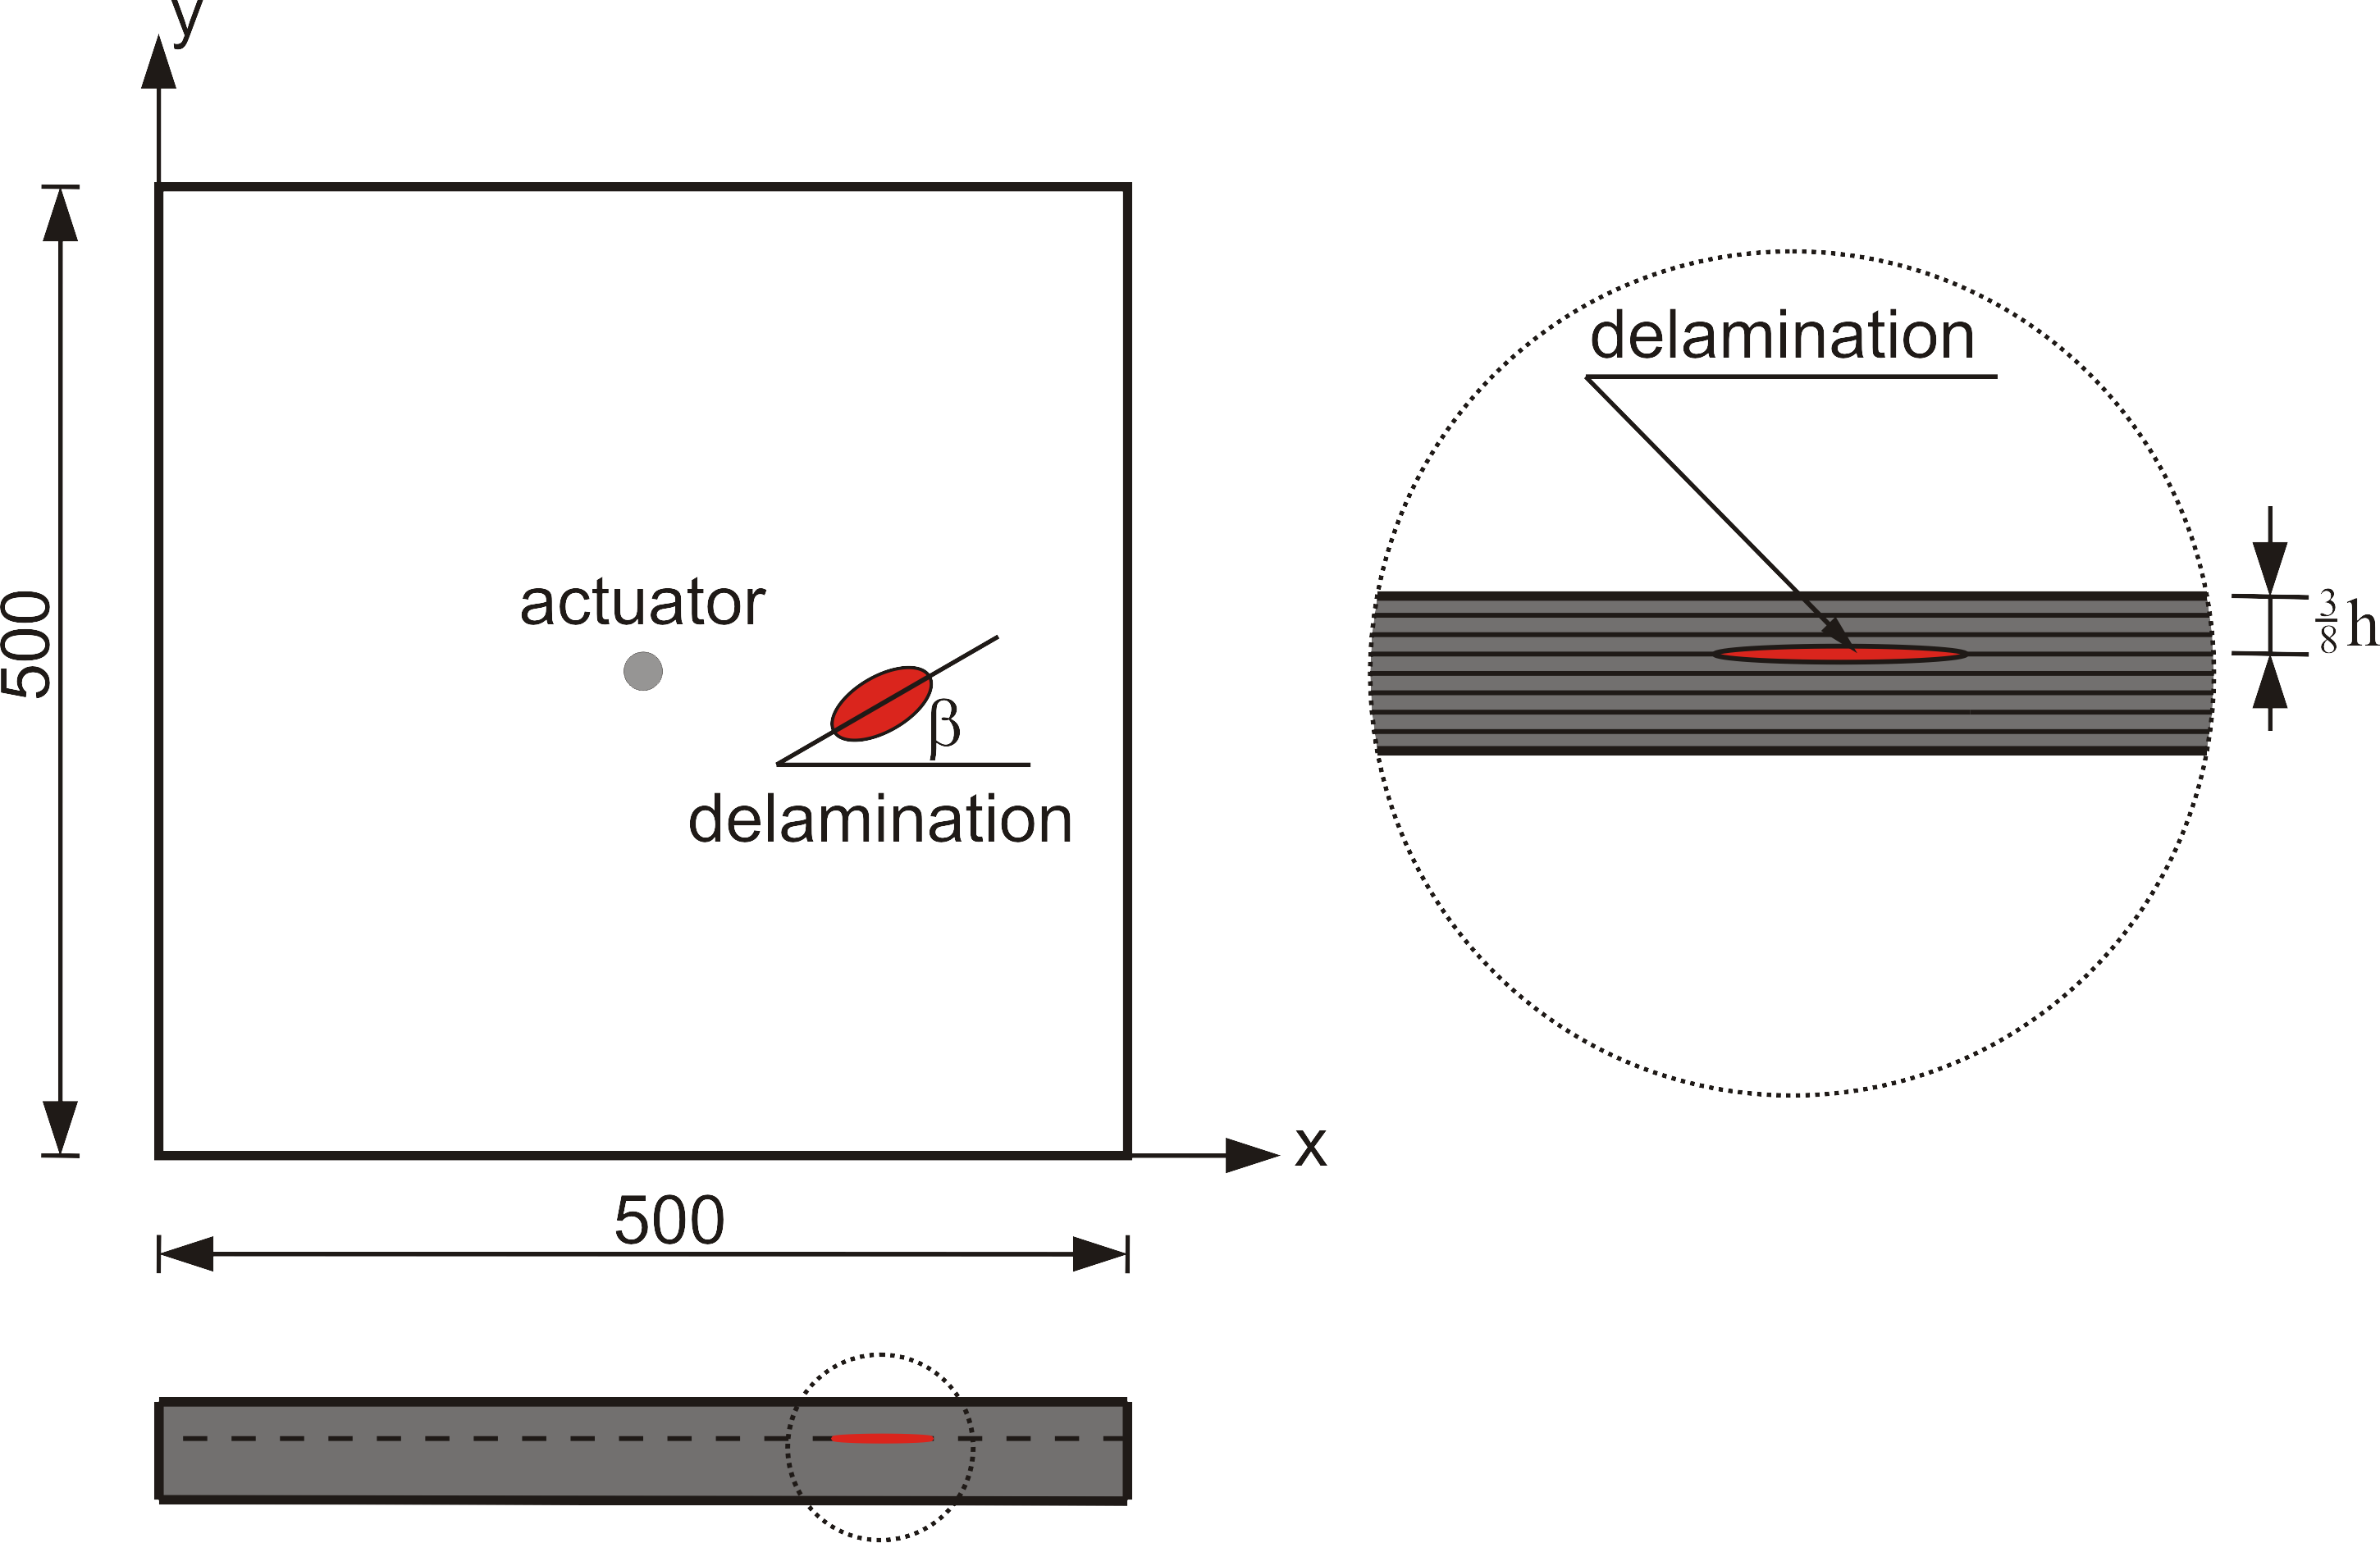
\includegraphics[scale=0.8]{plate_delam_arrangement_MSSP.png}
	\caption{Setup for computing Lamb wave interactions with delamination.}
	\label{fig:plate_setup}
\end{figure}	
\begin{figure}
	\centering
	\includegraphics[scale=1]{dataset2_labels_ellipses.png}
	\caption{The plate with 475 cases of random delaminations.}
	\label{fig:random_delam}
\end{figure}
		
Guided waves were excited at the plate centre by applying equivalent piezoelectric forces.
The excitation signal had a form of sinusoid modulated by Hann window. 
It was assumed that the carrier frequency is 50 kHz and the modulation frequency is 10 kHz.
A relatively low carrier frequency allowed for lower mesh density and significant computation time reduction in comparison to simulations of higher frequencies.
Additionally, the excitation signal was selected so that interaction of generated A0 Lamb wave mode with the smallest delamination can be still used as a feature for damage identification.

The output from the top and bottom surfaces of the plate in the form of particle velocities at the nodes of spectral elements were interpolated on the uniform grid of 500\(\times\)500 points by using shape functions of elements (see~\cite{Kudela2020} for more details).
It essentially resembles measurements acquired by SLDV in the transverse direction (perpendicular to the plate surface).
An example of the simulated full wavefield data on the top and bottom surfaces is presented in Fig.~\ref{fig:wavefield}.
It should be noted that stronger wave entrapment at delamination can be observed for the case of the wavefield at the top surface.
It is because the delamination within cross-section is located closer to the top surface.
It makes it easier to detect delamination by processing wavefield at the top surface.
It is better visible if the root mean square (RMS) according to Eq.~(\ref{eq:rms}) is applied to the wavefield.
The result of this operation is presented in Fig.~\ref{fig:rms}.
Based on the image analysis, the shape of the delamination can be easier to discern for the top case.
However, the methodology presented in this paper was applied to the more difficult case i.e. wavefield registered at the bottom surface of the plate.

The dataset consisting of RMS images which were used in this research paper is available online~\cite{Kudela2020d}.

\begin{figure} [h!]
	\centering
	\begin{subfigure}[b]{0.32\textwidth}
		\centering
		\includegraphics[scale=1]{96_flat_shell_Vz_1_500x500top.png}
		\caption{\(t=0.141\) ms}
		\label{fig:frame96top}
	\end{subfigure}
	\hfill
	\begin{subfigure}[b]{0.32\textwidth}
		\centering
		\includegraphics[scale=1]{128_flat_shell_Vz_1_500x500top.png}
		\caption{\(t=0.188\) ms}
		\label{fig:frame128top}
	\end{subfigure}
	\hfill
	\begin{subfigure}[b]{0.32\textwidth}
		\centering
		\includegraphics[scale=1]{164_flat_shell_Vz_1_500x500top.png}
		\caption{\(t=0.240\) ms}
		\label{fig:frame164top}
	\end{subfigure}	
	\hfill
	\begin{subfigure}[b]{0.32\textwidth}
		\centering
		\includegraphics[scale=1]{96_flat_shell_Vz_1_500x500bottom.png}
		\caption{\(t=0.141\) ms}
		\label{fig:frame96bottom}
	\end{subfigure}
	\hfill
	\begin{subfigure}[b]{0.32\textwidth}
		\centering
		\includegraphics[scale=1]{128_flat_shell_Vz_1_500x500bottom.png}
		\caption{\(t=0.188\) ms}
		\label{fig:frame128bottom}
	\end{subfigure}
	\hfill
	\begin{subfigure}[b]{0.32\textwidth}
		\centering
		\includegraphics[scale=1]{164_flat_shell_Vz_1_500x500bottom.png}
		\caption{\(t=0.240\) ms}
		\label{fig:frame164bottom}
	\end{subfigure}

	\caption{Full wavefield at the top surface (a)--(c) and the bottom surface (d)--(f), respectively, at selected time instances showing the interaction of guided waves with delamination.}
	\label{fig:wavefield}
\end{figure} 

\begin{figure} [h!]
	\centering
	\begin{subfigure}[b]{0.47\textwidth}
		\centering
		\includegraphics[scale=1]{RMS_flat_shell_Vz_1_500x500top.png}
		\caption{top}
		\label{fig:rmstop}
	\end{subfigure}
	\hfill
	\begin{subfigure}[b]{0.47\textwidth}
		\centering
		\includegraphics[scale=1]{RMS_flat_shell_Vz_1_500x500bottom.png}
		\caption{bottom}
		\label{fig:rmsbottom}
	\end{subfigure}
	\caption{RMS of the full wavefield from the top surface of the plate (a) and the bottom surface of the plate (b).}
\label{fig:rms}
\end{figure} 
%%%%%%%%%%%%%%%%%%%%%%%%%%%%%%%%%%%%%%%%%%%%%%%%%%%%
\subsection{Signal processing strategy}
%%%%%%%%%%%%%%%%%%%%%%%%%%%%%%%%%%%%%%%%%%%%%%%%%%%%
Two signal processing strategies are applied: newly proposed image processing based on the FCN and conventional one which is the adaptive wavenumber filtering.
The former one is represented by the left branch on the scheme shown in~Fig.~\ref{fig:sig_proc_strategy} whereas the latter one is represented by the right branch.
The starting point for both approaches is the dataset consisted of frames of propagating guided waves.
However, the FCN takes as an input the RMS which combines all frames into one image. 
It essentially represents the spatial energy distribution of propagating waves.
In the adaptive wavenumber filtering method, all frames are utilised (right branch of Fig.~\ref{fig:sig_proc_strategy}).
The RMS is applied later on to output final damage map in the form of an image.

It should be noted that we tested two types of activation functions as a last layer of the FCN: softmax and sigmoid.
The former one gives the binary output which segments pixels in two categories: damaged and undamaged.
On the other hand, the threshold needs to be applied when the sigmoid activation function is used.
Also, damage maps resulted from the adaptive wavenumber filtering must be thresholded so that the area and shape of delamination can be estimated.

Finally, IoU is applied as a measure of delamination size, shape and location so that all presented approaches can be compared quantitatively. 
	\begin{figure}
		\centering
		\includegraphics[scale=0.8]{FCN_adaptive_filtering_diagram_MSSP.png}
		\caption{Diagram of signal processing strategy by the proposed Fully Convolutional Network (left branch) in comparison to signal processing utilising adaptive wavenumber filtering method (right branch). }
		\label{fig:sig_proc_strategy}
	\end{figure}
The particular blocks presented in the Fig.~\ref{fig:sig_proc_strategy} will be explained in more details in the next sections.

%%%%%%%%%%%%%%%%%%%%%%%%%%%%%%%%%%%%%%%%%%%%%%%%%%%%	
\subsection{Adaptive wavenumber filtering}
%%%%%%%%%%%%%%%%%%%%%%%%%%%%%%%%%%%%%%%%%%%%%%%%%%%%
Adaptive wavenumber filtering is a well-established method for processing of images of propagating elastic waves.
The method has proved to be useful for crack size estimation~\cite{Kudela2015}, impact induced damage assessment~\cite{Kudela2018},  delamination and disbonding detection and localisation~\cite{Radzienski2019}.  
It is used here as a reference point for comparison purposes against proposed strategies based on FCN.

The method involves steps such as 2D Fourier Transform, wavenumber filtering, inverse Fourier Transform and RMS.
It can be used as an automated tool for producing damage maps which are easy in interpretation.
However, it still requires setting a threshold for the filter mask and quantisation threshold useful for damage size estimation.
These thresholds can be estimated empirically and even certain rigid range of thresholds will lead to satisfactory results.
Nevertheless, it is not a fully automatic process.
FCN based approach seems to have an advantage in this regard.
On the other hand, FCN would also need some prior inductive bias from the domain knowledge such as pre-processing parameters, supervision into assigned class, and the most important one: assumption that pixels of processed images can be categorized as damaged and undamaged.
Moreover, the training of FCN requires tuning of many hyperparameters such as  learning rate, momentum, choice of optimizer, dropout rate, batch size, etc. 
But this process must be completed only once.
%%%%%%%%%%%%%%%%%%%%%%%%%%%%%%%%%%%%%%%%%%%%%%%%%%%%%
\subsection{Fully Convolutional Network approach}
%%%%%%%%%%%%%%%%%%%%%%%%%%%%%%%%%%%%%%%%%%%%%%%%%%%%%
In this section, a deep learning approach for delamination detection in composite materials is presented. 
%%%%%%%%%%%%%%%%%%%%%%%%%%%%%%%%%%%%%%%%%%%%%%%%%%%%%
\subsubsection{Data preprocessing}
%%%%%%%%%%%%%%%%%%%%%%%%%%%%%%%%%%%%%%%%%%%%%%%%%%%%%
It should be noted that the output from the wave propagation model is in the form of a 3D matrix which contains amplitudes of propagating waves at location \((x, y)\) and time \(t\). We can look at it as a set of frames of propagating waves at discrete time moments \(t_k\).

The data preprocessing as it is indicated in Fig.~\ref{fig:sig_proc_strategy} include a step of computation of root mean square value:
\begin{equation}
	\hat{s}(x,y) = \sqrt{\frac{1}{N}\sum_{k=1}^{N} s(x,y,t_k)^2}
	\label{eq:rms}
\end{equation}
where the number of sampling points \(N\) was 512.
In this way, the dataset was collapsed to 475 2D matrices in which amplitudes are stored as double-precision values.
The next step was the conversion of these matrices to greyscale images (colour image quantisation).
Colour scale values of obtained images vary between (\(0 - 255\)) hence normalization
to a range of (\(0-1\)) was applied to improve convergence of gradient descent algorithm (Adam optimizer). 
	
Furthermore, data augmentation was achieved by flipping images horizontally, vertically and diagonally. 
It increased the dataset size four times -- \(1900\) images were produced.
Such data augmentation can enhance the learning process by enabling the model to learn and recognise new complex patterns.
	
The data set was split into two portions:  \(80\%\) for the training set and \(20\%\) for the testing set.
Additionally, the validation set was created as a \(20\%\) of the training set.

%%%%%%%%%%%%%%%%%%%%%%%%%%%%%%%%%%%%%%%%%%%%%%%%%%%%%
%%%%%%%%%%%%%%%%%%%%%%%%%%%%%%%%%%%%%%%%%%%%%%%%%%%%%
\subsubsection{The basic concept of Fully Convolutional Network}
%%%%%%%%%%%%%%%%%%%%%%%%%%%%%%%%%%%%%%%%%%%%%%%%%%%%%
The main purpose of such approach is to automatically perform feature extraction by training a model using full wavefield images, hence, it will learn by itself to recognise the patterns and detect the delamination and localise it.
In our work we are using the fully convolutional network (FCN)~\cite{long2015fully}, which aims to perform pixel-wise segmentation by classifying every pixel of the input image as damaged or not. 

The idea behind FCN is to stack a group of convolutional layers in an encoder-decoder style. 
The encoder is capable for downsampling the input image through convolutions with strides, consequently, resulting in a compressed feature representation of the input image, and the decoder is capable to upsample the image with compressed features applying techniques like transposed convolution with strides and upsampling with interpolation (e.g. bilinear or nearest).


In order to reduce overfitting in the model, some techniques were applied such as adding dropouts to layers and batch normalization.

For the output layer, we have applied two activation functions in separate experiments, the first one is softmax and the second one is sigmoid. 
The softmax function calculates the probability of the damage occurrence and the healthy state for every single pixel, hence, the summation of the two probabilities must equal one. Eq.~(\ref{softmax}) illustrates the softmax, where \(P(x)_{i}\) is the probability of each target class \(x_{j}\) over all possible target classes \(x_{j}\), C in our case are two classes  (damaged and undamaged).
To predict the output label of the detection (\(y_{pred}\)) which represent the probability of damaged and undamaged, we applied the \(\argmax\) function to select the maximum probability of the softmax activation function.
	\begin{equation}
		P(x)_{i} = \frac{e^{x_{i}}}{\sum_{j}^{C} e^{x_{j}}}
		\label{softmax}
	\end{equation} 
	\begin{equation}
		y_{pred} = \argmax_{i}\left( P(x)_{i} \right)
		\label{argmax}
	\end{equation}

When using sigmoid in the output layer, it produces a vector of values between (\(0\) and \(1\)) indicating the damage weight for each pixel. 
Low values indicate low damage probability and high output values indicate high damage probability. Eq.~(\ref{sigmoid}) illustrates the sigmoid function, where \(z\) is the summation of adjustable weights \(\{w_0,w_1,...,w_n \}\) multiplied by input variables (from the previous layer) \(\{x_0,x_1,_...,x_n\}\) and bias \(b\) as shown in Eq.~(\ref{z}).	
	\begin{equation}
		\sigma(z) = \frac{1}{1+e^{-z}}
		\label{sigmoid}
	\end{equation}
	\begin{equation}
		z= \sum_{i=0}^{n}  w_i\, x_i +b
		\label{z}
	\end{equation}
Selecting the loss function is a crucial task in deep learning since it measures how good the model predicts.
We have applied two types of losses based on the used function in the final activation layer: a binary cross-entropy (BCE) loss function applied with a sigmoid activation function in the output layer and a categorical cross-entropy (CCE) loss function with a softmax activation in the output layer that is also called \enquote{softmax loss function}.
Eq.~(\ref{BCE}) illustrates the BCE, where \(\hat{Y}\) represents the predicted vector values and \(Y\) represents the ground truth vector values, when \(\hat{Y} \approx Y\) then the BCE will be almost \(0\) meaning that the model was able to predict the output, so, the aim is to reduce the loss function to the minimum value.
	\begin{equation}
		BCE = (1-Y)\log(1-\hat{Y})+Y\log(\hat{Y})
		\label{BCE}
	\end{equation}
Eq.~(\ref{CCE}) illustrates the CCE, where \( P(x)_{i}\) is the softmax value of the target class. 
	\begin{equation}
	CCE = -\log\left( P(x)_{i} \right)
	\label{CCE}
	\end{equation}

Moreover, we have applied intersection over union (IoU) as our accuracy metric. 
IoU is applied to find the intersection area between the ground truth value and the predicted value.  
The IoU metric is defined as:
\begin{equation}
IoU = \frac{Intersection}{Union} = \frac{\hat{Y} \cap Y}{\hat{Y} \cup Y} 
\label{IoU}
\end{equation}
The intersection between the predicted and the ground truth values is simply calculated through multiplying their values then summing the resulted values.
As we mentioned earlier the ground truth values are either \((0\) or \(1)\) thus only the predicted values larger than \(0\) multiplied by their ground truth label \(1\) will be counted, the rest values will equal to \(0\). 
The union can be calculated by summing all values in both the predicted and the ground truth  vectors, then we subtract the intersection from their sum.
Our main goal is to maximize the IoU accuracy metric, since the higher the IoU, the higher the accuracy of the predicted delamination in terms of location, shape and size.
	
Furthermore, during training the model our focus is to minimize the loss and maximize the accuracy metric by converting it into an optimization problem. 
The optimizer is responsible for updating the model learnable parameters such as filters weights and biases in a way the overall loss is minimized and the accuracy is maximized.
In the proposed approach, Adam optimizer was applied, which is considered as a combination of RMSprop and Stochastic Gradient Descent (SGD)~\cite{Kingma2015}. 

In the next subsection, we are going to present an FCN model for pixel-wise semantic segmentation in order to detect and localise delaminations.

%%%%%%%%%%%%%%%%%%%%%%%%%%%%%%%%%%%%%%%%%%%%%%%%%%%%%
%\subsubsection{U-net based model}
%	%%%%%%%%%%%%%%%%%%%%%%%%%%%%%%%%%%%%%%%%%%%%%%%%%%%%
%	Our first FCN model is the U-net based-model, which was introduced by Ronneberger et al.~\cite{Ronneberger2015} for biomedical image segmentation constructed from two parts encoder and decoder. 
%	This architecture consists of three sections: The downsampling section, The bottleneck, and the upsampling section. 
%	The downsampling section holds several contraction blocks. 
%	Each block takes an input applies two (\(3\times3\)) convolution layers followed by a (\(2\times2\)) max pooling with a (\(2\times2\)) strides. 
%	The number of convolutional filters is doubled after each downsampling block so that architecture can learn the complex patterns effectively. 
%	The bottleneck layer meddles between the downsampling section and the upsampling section. 
%	It composed of two (\(3\times3\)) convolution layers followed by (\(2\times2\)) up convolution layer (Transpose convolution).
%	The upsampling section is similar to downsampling section, it also consists of several upsampling blocks. 
%	Each block passes the input to two (\(3\times3\)) convolution layers followed by a (\(2\times2\)) Convolutional transposed layer (upsampling). 
%	Moreover, after each block, the number of feature maps used by convolutional layer get half to keep the model symmetrical. 
%	Further, skip connections were added by appending feature maps of the downsampling block with the corresponding upsampling block to retrieve lost spatial information during the downsampling to due to decreasing the input resolution.
%	By doing so, the model ensures that the feature maps which were learned during the image downsampling will be utilised to reconstruct it. 
%	Furthermore, to enhance the model training performance we applied a technique called batch-normalization (BN)~\cite{Ioffe2015}.
%	The term "batch" was added because, during training, we normalize the output of the previous layer for each batch, applying a transformation that keeps the mean activation value close to \(0\) and the activation standard deviation close to \(1\), which eventually enhances the learning rate.
%	\begin{figure} [h!]
%		\begin{center}
%			\includegraphics[scale= 0.8]{Unet_model.png}
%		\end{center}
%		\caption{U-Net architecture.} 
%		\label{fig:Unet}
%	\end{figure}
%	Fig.~\ref{fig:Unet} presents the model architecture showing the path of the input of a full wavefield image of a size (\(512\times512\)) through the downsampling, bottleneck then the upsampling finally to the output which contains the prediction of delamination size and location. 
%	In the downsampling section,
%	Each layer performs (\(3\times3\)) convolution, followed by Relu activation function followed by BN operation.
%	Further, the Transmission Down layer contains a Maxpool function with (\(2\times2\)) pooling filter and a (\(2\times2\)) strides that picks the maximum value in a local pool filter in one feature map (or \(n\)-feature maps), resulting in a reduction in the dimension of feature maps~\cite{Lecun2015}, consequently, reducing computation complexity.
%	The bottleneck section is the deepest section in the model, it contains two convolutional layers, with 256 filters which helps the model to learn and recognize new complex patterns.
%	The Upsampling section is similar to the down sampling section, in which each layer  performs (\(3\times3\)) convolution, followed by Relu activation function followed by BN operation. But, for the Transmission Up layer it perform the opposite of downsampling.
%	The purpose is to retrieve the dimensions before sampling and increase the resolution of the images. 
%	For this model we have applied a (\(3\times3\))Transposed convolution with (\(2\times2\)) strides.
%	Transposed convolution layer differs from the regular upsampling function, by introducing learnable parameters regarding the transposed convolution filters that enhance the learning process of the model, therefore, new patterns are recognized. 
%	%%%%%%%%%%%%%%%%%%%%%%%%%%%%%%%%%%%%%%%%%%%%%%%%%%%%
	\subsubsection{FCN-DenseNet based model}
	%%%%%%%%%%%%%%%%%%%%%%%%%%%%%%%%%%%%%%%%%%%%%%%%%%%%%	
	FCN-DenseNet was introduced by Simon Jegou et al.~\cite{jegou2017one} for semantic segmentation.
	It is based on the DenseNet model originally proposed by Huang et al.~\cite{Huang}. 
	The main advantage of FCN-DenseNet over DenseNet is the extra utilising of feature maps by adding the upsampling path to the model.
	FCN-DenseNet is composed of downsampling path, upsampling path and skip connections.
	Skip connections from the downsampling path to the corresponding upsampling path are essential for recovering spatially detailed information by reusing feature maps.
 
	The essential component in FCN-DenseNet is a dense block.
	The purpose of the dense block is to concatenate layer input (feature maps) with its output (feature maps) to emphasize spatial details information.
	The dense block is constructed from \(n\) varying number of layers, each layer is composed of a series of operations.
	Figure~\ref{dense_block} presents the architecture of the dense block.
	It has an input (\(x\)) (input image or output of transition layer) with \(k\) feature maps which is concatenated with the output of first layer and this process is recursively performed for all layers in the dense block ending up with output (\(y\)) with a (\(n\times k\)) feature maps. 
	Transition down layer was introduced to reduce the spatial dimensionality of the feature maps by performing a (\(1\times 1\)) convolution followed by (\(2\times2\)) Maxpool operation. 

	\begin{figure} [h!]
		\begin{center}
			\includegraphics[scale=1,angle=-90]{fig6.png}
		\end{center}
		\caption{Dense block architecture.} 
		\label{dense_block}
	\end{figure}

	For the transition up layer, it was introduced in FCN-DenseNet to recover the input spatial resolution, to do that a transpose convolution operation is performed which upsamples the previous feature maps.
	Feature maps emerging from upsampling are concatenated with the ones resulting from the skip connection forming the input to a new dense block.
	During the upsampling, the input to the dense block is not concatenated with its output to overcome the overhead of memory shortage since the upsampling path expands the spatial resolution of the feature maps.
	Table~\ref{layers} presents the architecture of a single layer, the transition down  and transition up layers in details.

	\begin{table}[h!]
		\renewcommand{\arraystretch}{1.3}
		\centering
		\scriptsize
		\begin{tabular}{|c|l|c|l|c|}
			\cline{1-1} \cline{3-3} \cline{5-5}
			\textbf{Layer} &  & \textbf{Transition Down} &  & \textbf{Transition Up} \\ \cline{1-1} \cline{3-3} \cline{5-5} 
			Batch Normalization &  & Batch Normalization &  & \multirow{5}{*}{\begin{tabular}[c]{@{}c@{}}(\(3\times3\)) Transposed Convolution, \\ strides = (\(2\times2\))\end{tabular}} \\ \cline{1-1} \cline{3-3}
			Relu &  & Relu &  &  \\ \cline{1-1} \cline{3-3}
			(\(3\times3\)) Convolution &  & (\(1\times1\)) Convolution &  &  \\ \cline{1-1} \cline{3-3}
			\multirow{2}{*}{Dropout \(p = 0.2\)} &  & Dropout \(p = 0.2\) &  &  \\ \cline{3-3}
			&  & (\(2\times2\)) Maxpooling &  &  \\ \cline{1-1} \cline{3-3} \cline{5-5} 
		\end{tabular}
		\caption{Layer, Transition Down and Transition Up layers.} 
		\label{layers}
	\end{table}

Figure~\ref{fcn} illustrates the FCN-DenseNet architecture for image segmentation used for delamination detection.
\begin{figure} [h!]
	\begin{center}
		\includegraphics[scale= 1]{fig7.png}
	\end{center}
	\caption{FCN-DenseNet architecture.} 
	\label{fcn}
\end{figure}
Our constructed model is composed of \(3\) dense blocks in the downsampling path, one dense block in bottleneck and 3 dense blocks for the upsampling path. 
Each dense block in the downsampling and upsampling paths consists of \(2\) layers, the bottleneck dense block consists of \(4\) layers.
The model input is the RMS image with size of (\(512\times 512\)).
At the beginning, we perform a  convolution operation and concatenate the original input with the output, then the concatenated output is fed into the first dense block that consists of (\(2\)) layers.

Each layer is composed of batch normalization (BN) followed by Relu, then (\(3\times3\)) convolution with same padding is applied followed by a dropout with probability \(p = 0.2\).
Then, the output of the first dense layer is concatenated with its input and is fed into a transition down layer. 

The transition down layer is composed of BN followed by Relu, then (\(1\times1\)) convolution followed by a dropout with probability \(p = 0.2\) and finally (\(2\times2\)) Maxpool with strides of (\(2\times2\)).

This process is repeated until the bottleneck dense block.
The bottleneck dense block consists of 4 layers.
The output of the bottleneck is directed into the upsampling path starting with transition up layer.
Accordingly, the output of the transition up layer is concatenated with the corresponding dense block output in the downsampling path.
The final layer in the network is  (\(1\times1\)) convolution followed by either a sigmoid function or a softmax function to calculate the probability of damage for each pixel.
Hence, we have two versions of the FCN-DenseNet model with different output layer function.


%	%%%%%%%%%%%%%%%%%%%%%%%%%%%%%%%%%%%%%%%%%%%%%%%%%%%%%
%	\subsubsection{FCN-VGG16}
%	%%%%%%%%%%%%%%%%%%%%%%%%%%%%%%%%%%%%%%%%%%%%%%%%%%%%%
%	In this model we address the use of VGG16-based encoder~\cite{Simonyan2015} with 13-convolutional layers.
%	VGG16 encoder is composed of convolutional layers, pooling layers and dense layers, and it was used for classification purposes. 
%	In our last model, we employed an encoder decoder scheme for pixel wise image segmentation. 
%	Both encoder and decoder layers were trained from scratch.
%	Figure~\ref{vgg16} presents the architecture of VGG16- encoder decoder model. 
%	The model consists of two paths: downsampling and upsampling.
%	The downsampling path consists of \(5\) convolutional blocks,  with a total \(13\) convolutional layers  with same padding and kernel size (\(3\times3\))and 32 filters for each layer, followed by BN and activation function Relu.
%	Each convolutional layer is responsible for extracting high level features from the input image such as edges.
%	A Maxpool operation with pool size of (\(2\times2\))  and (\(2\times2\)) strides followed by dropout is performed after each convolutional block. 
%	The upsampling path is introduced to recover spatial resolution, it also has \(5\) convolutional blocks with a total \(13\) convolutional layers  with same padding and kernel size (\(3\times3\))and 32 filters for each layer, followed by BN and activation function Relu.
%	For upsampling, bilinear interpolation with (\(2\times2\)) kernel size is applied.
%	Skip connections were added between downsampling blocks and the corresponding upsampling blocks in order to enhance recovering fine-grained details by enabling feature re-usability from earlier layers.
%	\begin{figure} [h!]
%		\begin{center}
%			\includegraphics[scale=0.8]{VGG16_encoder_decoder.png}
%		\end{center}
%		\caption{VGG16 encoder decoder architecture.} 
%		\label{vgg16}
%	\end{figure}

%%%%%%%%%%%%%%%%%%%%%%%%%%%%%%%%%%%%%%%%%%%%%%%%%%%%%
\section{Results and Discussions}
%%%%%%%%%%%%%%%%%%%%%%%%%%%%%%%%%%%%%%%%%%%%%%%%%%%%%
In this section, we are going to show some results for delamination detection in accordance with the adaptive wavenumber filtering and the FCN-DenseNet model. 
%	As we mentioned earlier, a sigmoid and a softmax functions are used at the output layer for our model, hence we have two versions of the FCN-DenseNet model with different output layer function.
	
The sigmoid function at the output layer of the FCN-DenseNet model computes the damage probability for each pixel, hence the damage probability ranges from (\(0 - 1\)).
Therefore, there is a need for a threshold function to exclude low probabilities of predicted damage. 
For all the following results, the threshold \(tr = 0.5\) was set, therefore any value less than \(0.5\) will be excluded from the damage map.
For the softmax function at the output layer, it computes two probabilities for each pixel: (damaged and undamaged), then an \(\argmax\) function is applied to select the highest probability between the two probabilities, therefore there is no need for thresholding. 
The FCN-DenseNet models was trained on augmented dataset up to 100 epochs, and the architecture of the FCN-DenseNet  was implemented using the open-source platform of Keras API~\cite{chollet2015keras} running on top of TensorFlow on a GeForce RTX 2080  GPU from NVIDIA.
For all scenarios, we selected a red colour to represent the detected delamination (damaged), and the blue colour to represent the healthy state (undamaged).
	
In the following, we are going to present three scenarios of delaminations of different locations, shapes and angles.

Figure~\ref{fig:RMS_flat_shell_Vz_438} shows the RMS of full wavefield interpolated at the bottom surface of the plate with delamination located at the top edge of the plate.
Figure~\ref{fig:m1_rand_single_delam_438} shows the ground truth image corresponding to Fig.~\ref{fig:RMS_flat_shell_Vz_438}. 
Fig.~\ref{fig:ERMSF_flat_shell_Vz_438} shows the detected delamination using the adaptive wavenumber filtering. 
The damage map represents the energy-based root mean square index of frames filtered in the wavenumber domain (ERMSF). 
It can be seen in the damage map that the delamination is detected, but still, the method boosts edge reflections which results in some noise at the edges. 
To eliminate low values from the ERMSF, a binary threshold is applied as shown in Fig.~\ref{fig:Binary_ERMSF_flat_shell_Vz_438}.
The threshold level was selected to limit the influence of edge noise and at the same time highlight the damage. 
The binary ERMSF properly indicates the location of delamination but still, there is some noise at the corners.
It results in the calculated IoU equal (\(0.10\)).
In Figs.~\ref{fig:predict_438_sigmoid_tr_0.5}, ~\ref{fig:predict_438_softmax} we present the FCN-DenseNet outputs with sigmoid and softmax respectively.
As shown, the FCN-DenseNet models detect the delamination without any noise at the edges as the FCN-DenseNet learned the delamination patterns from the large numerically generated dataset and can differentiate among different complex patterns such as noise.   
The IoU = \(0.73\) for sigmoid, and IoU = \(0.65\) for the softmax.
	%%%%%%%%%%%%%%%%%%%%%%%%%%%%%%%%%%%%%%%%%%%%%%%%%%%
	%first figure
	%%%%%%%%%%%%%%%%%%%%%%%%%%%%%%%%%%%%%%%%%%%%%%%%%%%
	\begin{figure} [!h]
		\centering
		\begin{subfigure}[b]{0.47\textwidth}
			\centering
			\includegraphics[scale=1]{RMS_flat_shell_Vz_438_500x500bottom.png}
			\caption{RMS bottom}
			\label{fig:RMS_flat_shell_Vz_438}
		\end{subfigure}
		\hfill
			\begin{subfigure}[b]{0.47\textwidth}
			\centering
			\includegraphics[scale=1]{m1_rand_single_delam_438.png}
			\caption{Ground truth}
			\label{fig:m1_rand_single_delam_438}
		\end{subfigure}
		\hfill
		\begin{subfigure}[b]{0.47\textwidth}
			\centering
			\includegraphics[scale=1]{ERMSF_flat_shell_Vz_438_500x500bottom.png}
			\caption{Adaptive wavenumber filtering (ERMSF)}
			\label{fig:ERMSF_flat_shell_Vz_438}
		\end{subfigure}
		\hfill
		\begin{subfigure}[b]{0.47\textwidth}
			\centering
			\includegraphics[scale=1]{Binary_ERMSF_flat_shell_Vz_438_500x500bottom.png}
			\caption{binary ERMSF}
			\label{fig:Binary_ERMSF_flat_shell_Vz_438}
		\end{subfigure}
		\hfill
		\begin{subfigure}[b]{0.47\textwidth}
			\centering
		\includegraphics[scale=1]{FCN_DenseNet_Predicted_438_sigmoid_thresholded_0.5.png}
		\caption{sigmoid \((tr = 0.5)\)}
		\label{fig:predict_438_sigmoid_tr_0.5}
		\end{subfigure}
		\hfill
		\begin{subfigure}[b]{0.47\textwidth}
			\centering
			\includegraphics[scale=1]{FCN_DenseNet_Predicted_438_softmax.png}
			\caption{softmax}
			\label{fig:predict_438_softmax}
		\end{subfigure}
		\caption{First delamination scenario based on numerical data.}
		\label{fig:RMS438}
	\end{figure} 
	%%%%%%%%%%%%%%%%%%%%%%%%%%%%%%%%%%%%%%%%%%%%%%%%%%%
	
In the next scenario, we present delamination located in the upper left part of the plate.
Figs.~\ref{fig:dispersion30deg_direct}, ~\ref{fig:m1_rand_single_delam_454} show the RMS of the full wavefield interpolated at the bottom surface of the plate.
Fig.~\ref{fig:ERMSF_flat_shell_Vz_454} shows the damage map obtained by using the adaptive wavenumber filtering.
The adaptive wavenumber filtering method picks some noise at the edges but the shape of delamination is clearly highlighted by high values of damage map.
Nevertheless, there is still some noise after applying threshold as it is shown in Fig.~\ref{fig:Binary_ERMSF}.
The IoU for this case is \(0.61\).
In Figs.~\ref{fig:predict_454_sigmoid_tr_0.5}, ~\ref{fig:predict_454_softmax} we present the FCN-DeneseNet outputs with sigmoid and softmax, respectively.
The sigmoid detect the delamination with IoU = \(0.58\), and for the softmax with IoU = \(0.60\).
As we can see also for this scenario, the FCN-DenseNet only detects the delamination patterns without unwanted noise.
%%%%%%%%%%%%%%%%%%%%%%%%%%%%%%%%%%%%%%%%%%%%%%%%%%%
	\begin{figure} [!h]
		\centering
		\begin{subfigure}[b]{0.47\textwidth}
			\centering
			\includegraphics[scale=1]{RMS_flat_shell_Vz_454_500x500bottom.png}
			\caption{RMS bottom}
			\label{fig:dispersion30deg_direct}
		\end{subfigure}
		\hfill
		\begin{subfigure}[b]{0.47\textwidth}
			\centering
			\includegraphics[scale=1]{m1_rand_single_delam_454.png}
			\caption{Ground truth}
			\label{fig:m1_rand_single_delam_454}
		\end{subfigure}
		\hfill
		\begin{subfigure}[b]{0.47\textwidth}
			\centering
			\includegraphics[scale=1]{ERMSF_flat_shell_Vz_454_500x500bottom.png}
			\caption{Adaptive wavenumber filtering (ERMSF)}
			\label{fig:ERMSF_flat_shell_Vz_454}
		\end{subfigure}
		\hfill
		\begin{subfigure}[b]{0.47\textwidth}
			\centering
			\includegraphics[scale=1]{Binary_ERMSF_flat_shell_Vz_454_500x500bottom.png}
			\caption{Binary ERMSF}
			\label{fig:Binary_ERMSF}
		\end{subfigure}
		\hfill
		\begin{subfigure}[b]{0.47\textwidth}
			\centering
			\includegraphics[scale=1]{FCN_DenseNet_Predicted_454_sigmoid_thresholded_0.5.png}
			\caption{sigmoid (tr =\(0.5\))}
			\label{fig:predict_454_sigmoid_tr_0.5}
		\end{subfigure}
		\hfill	
		\begin{subfigure}[b]{0.47\textwidth}
			\centering
			\includegraphics[scale=1]{FCN_DenseNet_Predicted_454_softmax.png}
			\caption{softmax}
			\label{fig:predict_454_softmax}
		\end{subfigure}
		\caption{Second delamination scenario based on numerical data.}
		\label{fig:RMS454}
	\end{figure} 
%%%%%%%%%%%%%%%%%%%%%%%%%%%%%%%%%%%%%%%%%%%%%%%%%%%	
%	Figs.[~\ref{fig:unthresholded438}, ~\ref{fig:unthresholded454}] show the original damage maps without thresholding for the FCN-DenseNet with sigmoid function for the first and second scenarios respectively. 
%	As shown from the figs, the predicted output has a range or probabilities of damage. 
%	Accordingly, we apply threshold to exclude these low damage probabilities.
%	\begin{figure} [!h] 
%		\centering
%		\begin{subfigure}[b]{0.47\textwidth}
%		\centering
%		\includegraphics[scale=1]{sigmoid_unthresholded438.png}
%		\caption{}
%		\label{fig:unthresholded438}
%		\end{subfigure}
%	\hfill	
%	\begin{subfigure}[b]{0.47\textwidth}
%		\centering 	
%		\includegraphics[scale=1]{sigmoid_unthresholded454.png}
%		\caption{}
%		\label{fig:unthresholded454}
%	\end{subfigure}
%	\caption{Unthresholded damage maps for FCN-DenseNet/sigmoid}
%	\label{fig:unthresholded}
%	\end{figure}

In Fig.~\ref{fig:RMS433} we present the third scenario where the damage map obtained by the adaptive wavenumber filtering method is useful for delamination visualisation but the FCN-DenseNet model failed.
%%%%%%%%%%%%%%%%%%%%%%%%%%%%%%%%%%%%%%%%%%%%%%%%%%%
% third figure
%%%%%%%%%%%%%%%%%%%%%%%%%%%%%%%%%%%%%%%%%%%%%%%%%%%
\begin{figure}[!h]
	\centering
	\begin{subfigure}[b]{0.47\textwidth}
		\centering
		\includegraphics[scale=1]{RMS_flat_shell_Vz_433_500x500bottom.png}
		\caption{RMS bottom}
		\label{fig:RMS_flat_shell_Vz_433}
	\end{subfigure}
	\hfill
	\begin{subfigure}[b]{0.47\textwidth}
		\centering
		\includegraphics[scale=1]{m1_rand_single_delam_433.png}
		\caption{ground truth}
		\label{fig:m1_rand_single_delam_433}
	\end{subfigure}
	\hfill
	\begin{subfigure}[b]{0.47\textwidth}
		\centering
		\includegraphics[scale=1]{ERMSF_flat_shell_Vz_433_500x500bottom.png}
		\caption{Adaptive wavenumber filtering (ERMSF)}
		\label{fig:ERMSF_flat_shell_Vz_433}
	\end{subfigure}
	\hfill
	\begin{subfigure}[b]{0.47\textwidth}
		\centering
		\includegraphics[scale=1]{Binary_ERMSF_flat_shell_Vz_433_500x500bottom.png}
		\caption{binary ERMSF}
		\label{fig:Binary_ERMSF_flat_shell_Vz_433}
	\end{subfigure}
	\caption{Third delamination scenario based on numerical data.}
	\label{fig:RMS433}
\end{figure} 

Figures.~\ref{fig:RMS_flat_shell_Vz_433}, ~\ref{fig:m1_rand_single_delam_433} show the RMS of the full wavefield interpolated at the bottom surface of the plate with delamination located at the upper left corner of the plate and its corresponding ground truth, respectively.
It is impossible to notice any changes of RMS pattern caused by the delamination (Fig.~\ref{fig:RMS_flat_shell_Vz_433}).
It should be noted that this image is fed to the FCN-DenseNet model whereas the full wavefield (all frames) are used in the adaptive wavenumber filtering method.
In extreme cases, like this, conventional signal processing has an advantage over the FCN-DenseNet model.
As shown in Fig.~\ref{fig:ERMSF_flat_shell_Vz_433} representing the damage map obtained by the adaptive wavenumber filtering technique, the delamination location can be identified by a well-trained expert. 
However, the values of the damage map corresponding to the delamination location are on the same level as the noise.
Hence, when binary thresholding is applied, only some false damage indications are highlighted near corners of the plate as show in Fig.~\ref{fig:Binary_ERMSF_flat_shell_Vz_433}. 
For this case IoU= \(0\) for all considered methods.
 
Delaminations located near edges or corners are difficult to detect due to edge wave reflections which have similar patterns as delamination reflections. 
The problem arises for both conventional and deep learning techniques. 
However, to solve this issue for the FCN model, we need to enhance the feature extraction process by obtaining more data to train the model to recognise and learn new patterns.	

In Table~\ref{tab:iou} we present the maximum, minimum and mean value of IoU for the adaptive filtering and FCN-DenseNet for sigmoid (threshold = \(0.5\)) and softmax for all testing images.
	\begin{table}
	 \renewcommand{\arraystretch}{1.3}
		\centering
		\caption{IoU for all models}
		\label{tab:iou}
		\resizebox{\textwidth}{!}{\begin{tabular}{ccccccccccccc}
				\toprule
				&  &  &  &  &  & \multicolumn{7}{c}{FCN-Dense Model} \\ \cline{7-13} 
				&  & \multicolumn{3}{c}{Adaptive filtering} &  & \multicolumn{3}{c}{sigmoid} &  & \multicolumn{3}{c}{softmax} \\ \cline{3-5} \cline{7-9} \cline{11-13} 
				&  & min & max & mean &  & min & max & mean &  & \multicolumn{1}{c}{min} & \multicolumn{1}{c}{max} & \multicolumn{1}{c}{mean} 
				%\\ \cline{3-13} 
				\\ \cline{3-5} \cline{7-9} \cline{11-13} 
				\multicolumn{2}{c}{IoU} &0&0.648&0.373& &0&0.933&0.616&  &0&0.878&0.623\\ 
				\bottomrule
		\end{tabular}}
	\end{table}
	
Every single value of the IoU was estimated for all testing images using FCN-DenseNet with a sigmoid at the output layers.
It is expected that as we increase the threshold, the IoU will decrease because some of the detected output values will be excluded.
Therefore, selecting the proper threshold value is important for maximizing IoU, and this is the reason why inductive bias is important. 
Fig.~\ref{fig:iou_fcn} shows the maximum and mean IoU for all testing images depending on the threshold value. 
The IoU is decreasing along with the threshold increment in the range of (\(0-1\)).
	\begin{figure}[!h] 
		\centering
		\includegraphics[width=\textwidth]{fcn_densenet_iou.png}
		\centering
		\caption{IoU for FCN-DenseNet with sigmoid of a range of thresholds \([0-1]\)} 
		\label{fig:iou_fcn}
	\end{figure}
	
In Fig.~\ref{fig:Exp_ERMS_teflon}, we present an experimental scenario of CFRP with Teflon insert as artificial delamination.
Similarly to the numerical case, the frequency of \(50\) kHz was used to excite the transducer which was placed at the centre of the plate.
As shown in Fig.~\ref{fig:ERMSF_CFRP_teflon} the adaptive wavenumber filtering method is able to detect the delamination. 
Fig.~\ref{fig:Binary_ERMSF_CFRP} shows the binary thresholded output which precisely highlights the location of delamination. 
Even the shape of the delamination is quite well represented.
The IoU for this scenario was \(0.401\). 

The FCN-DenseNet model detected the delamination with both a sigmoid and softmax functions as shown in Fig.~\ref{fig:EXP_predict_sigmoid} and Fig.~\ref{fig:EXP_predict_softmax}, respectively.
The IoU for FCN-DenseNet model was \(0.053\) and \(0.081\) for a sigmoid and softmax, respectively.
These poor results of predictions are expected since we trained our model only on numerically generated data.
However, apart from the noise at the edges and at the transducer location, the FCN-DenseNet could detect the delamination in the experimentally generated image.
It means that the model has excellent generalisation capabilities and is able to detect delamination based on previously unseen data.
We expect, that the generalisation capabilities and, in turn, delamination identification performance, can be further enhanced by training the model on experimental data.
However, the generation of large dataset comprised of experiments with various defects is troublesome.
	\begin{figure} [!h]
		\centering
		\begin{subfigure}[b]{0.47\textwidth}
			\centering
			\includegraphics[scale=1]{ERMS_CFRP_teflon_3o_375_375p_50kHz_5HC_x12_15Vpp.png}
			\caption{ERMS CFRP Teflon inserted}
			\label{fig:Delamination}
		\end{subfigure}			
		\hfill
		\begin{subfigure}[b]{0.47\textwidth}
			\centering 	
			\includegraphics[scale=1]{label_CFRP_teflon_3o_375_375p_50kHz_5HC_x12_15Vpp.png}
			\caption{Ground truth} 
			\label{fig:damage_label}
		\end{subfigure}
		\hfill
		\begin{subfigure}[b]{0.47\textwidth}
			\centering
			\includegraphics[scale=1]{ERMSF_CFRP_teflon_3o_375_375p_50kHz_5HC_x12_15Vpp.png}
			\caption{ERMSF} 
			\label{fig:ERMSF_CFRP_teflon}
		\end{subfigure}
		\hfill
		\begin{subfigure}[b]{0.47\textwidth}
		\centering
		\includegraphics[scale=1]{Binary_ERMSF_CFRP_teflon_3o_375_375p_50kHz_5HC_x12_15Vpp.png}
		\caption{Binary ERMSF} 
		\label{fig:Binary_ERMSF_CFRP}
		\end{subfigure}
		\hfill
		\begin{subfigure}[b]{0.47\textwidth}
			\centering
			\includegraphics[scale=1]{Predicted_Predicted_ERMS_CFRP_teflon_3o_375_375p_50kHz_5HC_x12_15Vpp_7__threshold_0.5_sigmoid.png}
			\caption{FCN DenseNet: sigmoid \((tr = 0.5)\)} 
			\label{fig:EXP_predict_sigmoid}
		\end{subfigure}
		\hfill
		\begin{subfigure}[b]{0.47\textwidth}
			\centering
			\includegraphics[scale=1]{Predicted_Predicted_ERMS_CFRP_teflon_3o_375_375p_50kHz_5HC_x12_15Vpp_7_softmax.png}
			\caption{FCN DenseNet: softmax} 
			\label{fig:EXP_predict_softmax}
		\end{subfigure}
			\caption{Experimental results}
			\label{fig:Exp_ERMS_teflon}
		\end{figure}
%%%%%%%%%%%%%%%%%%%%%%
%%%%%%%%%%%%%%%%%%%%%%%%%%%%%%%%%%%%%%%%%%%%%%%%%%%%%
%%%%%%%%%%%%%%%%%%%%%%%%%%%%%%%%%%%%%%%%%%%%%%%%%%
\section{Conclusions}
%%%%%%%%%%%%%%%%%%%%%%%%%%%%%%%%%%%%%%%%%%%%%%%%%%
In this paper, we addressed delamination detection in composite materials using a deep learning technique. 
For this purpose, we have trained an FCN-DenseNet for semantic segmentation on a numerically generated data -- simulated full wavefield of propagating guided waves.
To see the feasibility of such a study, we have compared the deep learning model with adaptive wavenumber filtering technique.
The results were promising, and the deep learning model surpasses the conventional technique in detecting the delaminations of different shapes, sizes and angles. 
Further, the model can be improved by training it on new experimental data.
It means that new patterns will be learned, hence it will enhance its ability to differentiate among various complex patterns.
Currently, our work focuses on delamination identification, however, it can be extended to the identification of different types of damage in composite materials.

In future, we are planning to implement several deep learning architectures to perform a comparative study of various deep learning models regarding delamination identification in composite materials.
\clearpage	
%\appendix
\section*{Acknowledgements}
The research was funded by the Polish National Science Center under grant agreement no 2018/31/B/ST8/00454.
We would like to acknowledge dr Maciej Radzienski for providing the experimental data of full wavefield measured by SLDV.

\bibliography{MSSP_Paper_final}
\bibliographystyle{num_order}
%\bibliographystyle{plain}
\end{document}


